\chapter{Home network management scalability} \label{sec:homework} 

\ifpdf
\graphicspath{{Chapter2/Chapter2Figs/PNG/}{Chapter2/Chapter2Figs/PDF/}{Chapter2/Chapter2Figs/}}
\else 
\graphicspath{{Chapter2/Chapter2Figs/EPS/}{Chapter2/Chapter2Figs/}} 
\fi

In this chapter we explore applications of the SDN technology to scale network
management in home networks. Drawing conclusions from existing social and user
studies, we identify a series of user management requirements and we  
redesign the home network functionality and control abstraction addressing these
requirements. We present a Strawman implementation of a network design which
achieves simplicity and scalability of the control abstraction within the home
environment. Additionally, we propose an extension of our design, which bridges
the gap between the home network users performance requirements and the ISP
resource allocation policy, providing a simple, scalable and user-friendly QoS
mechanism.

In this chapter, motivated by the nature of the problems and the inherent
opportunities of home networks (Section~\ref{s:evolution}),  we present a home
router design~(Section~\ref{s:router}) and evaluate a number of proposed
protocol modifications placing the homeowner in direct control of their
network~(Section~\ref{s:protocols}). In addition, we present a simple QoS
mechanism enabling user-ISP collaboration to improve resource utilisation in the
last-mile bottleneck of the ISP (Section~\ref{s:qos}). Finally we conclude
the results of our exploration~(Section~\ref{s:conclusion}).

Note that throughout this Chapter we refer to the individual managing the home
network as the homeowner without loss of generality; clearly any suitably
authorised member of the household, owner or not, may be able to exercise control
based on specifics of the local context. 

\section{Motivations}\label{s:evolution}

In this section we elaborate on the nature of the problems and opportunities
inherent to home networks. We motivate motivate our thesis by presenting the
findings of relevant ethnographic and social studies
(Section~\ref{sec:homework:use_cases}) and set the requirements for our system
(Section~\ref{s:revolution}). 

\subsection{Home Network: Use cases} \label{sec:homework:use_cases}

Many empirical studies in recent years have explored the clear mismatch between
current networking technology and the needs of the domestic setting,  in both
the
UK~\mycite{tolmie07,rodden07,rodden04,crabtree03}
and the
US~\mycite{shehan07,grinter05,sung07,chetty07,shehanpoole08}.
These studies present a weight of evidence that problems with home networking
are not amenable to solution via a `thin veneer' of user interface technology
layered atop the existing architecture.  Rather, they are \emph{structural},
emerging from the mismatch between the stable `end-to-end' nature of
the Internet and the highly dynamic and evolving nature of domestic
environments.  

Home networks use the same protocols, architectures, and tools once developed
for the Internet in the 1970s.  Inherent to the Internet's `end-to-end'
architecture is the notion that the core is simple and stable, providing only a
semantically neutral transport service.  The core protocols were designed for a
certain context of \emph{use} (assuming relatively trustworthy endpoints), made
assumptions about \emph{users} (skilled network and systems administrators both
using connected hosts and running the network core), and tried to accomplish a
set of \emph{goals} (e.g.,~scalability to millions of nodes) that simply do not
apply in a home network. 

In fact, the home network is quite different in nature to both core and
enterprise networks.  Existing studies~\mycite{tolmie07,shehan07,shehanpoole08}
suggest domestic networks tend to be relatively small in size with between 5 and
20 devices connected at a time.  The infrastructure is predominately
cooperatively self-managed by residents who are seldom expert in networking
management and, as this is not a professional activity, rarely motivated to
become expert.  A wide range of devices connect to the home network, including
desktop PCs, games consoles, and a variety of mobile devices ranging from
smartphones to digital cameras.  Not only do these devices vary in capability,
they are often owned and controlled by different household members.  

To illustrate the situation we are addressing, consider the following three
example scenarios, drawn from  situations that emerged from fieldwork 
reported in more detail elsewhere~\mycite{wmust2011,Chetty10}: 

\begin{quote}
\textbf{Negotiating acceptable use}.  William and Mary have a spare room which
they let to a lodger, Roberto.  They are not heavy network users and so,
although they have a wireless network installed, they pay only for the lowest
tier of service and they allow Roberto to make use of it.  The lowest tier of
service comes under an acceptable use policy that applies a monthly bandwidth
cap.  Since Roberto arrived from Chile they have exceeded their monthly cap on
several occasions, causing them some inconvenience.  They presume it is
Roberto's network use causing this, but are unsure and do not want to cause
offence by accusing him without evidence.
\end{quote}

\begin{quote}
\textbf{Welcome visitors, unwelcome laptops}.  Steve visits his friends Mike and
Elisabeth for the weekend and brings his laptop and smartphone.  Mike has
installed several wireless access points throughout his home and has secured the
network using MAC address filtering in addition to WPA2.  To access the network,
Steve must not only enter the WPA2 passphrase, but must also obtain the MAC
addresses of his devices for Mike to enter on each wireless access point.  Steve
apologizes for the trouble this would cause and, rather than be a problem to his
hosts, suggests he reads his email at a local cafe.
\end{quote}

\begin{quote}
\textbf{Socially efficient network sharing}.  Richard, the teenage son of Derek
exhibits a great interest in online Music services. Derek works some times from
home, using the Terminal Services provided by his employee. Tension is created
between the household members,  as Derek blames Richard downloading activity for
his poor performing remote desktop application. 
\end{quote}

In such ways, simple domestic activities have deep implications for
infrastructures that generate prohibitive technical overheads.  In the first
scenario, the problem is simply that the network's behaviour is opaque and
difficult for normal users to inspect; in the second, the problems arise from
the need to control access to the network and the technology details exposed by
current mechanisms for doing so; in the third, the problem arises from the
inability of the resource allocation algorithm to capture the social aspect of
the home setting.  

Home networks enable provision of a wide range of services, e.g.,~file stores,
printers, shared Internet access, music distribution.  The broad range of
supported activities, often blending work and leisure, make network use very
fluid.  In turn, this makes it very hard to express explicitly \emph{a priori}
policies governing access control or resource management~\mycite{tolmie07}.
Indeed, fluidity of use is such that access control and policy may not even be
consistent, as network management is contingent on the household's immediate
needs and routines.

\subsection{Home Networks: Revolution!} \label{s:revolution}

Current network functionality is spread across multiple layers that implement
different abstractions, while multiple protocols are used to allow network hosts
to communication over these layers. Each layer exposes a different set of
control parameters and effective network management \emph{must} exercise control
on multiple layers. Ultimately, this control distribution architecture is not
scalable for the average user. Simply creating a user interface layer for the
existing network infrastructure will only reify existing problems.  Rather, we
need to investigate creation of new network architectures reflecting the
socio-technical nature of the home by taking into account both human and
technical considerations. Control of the network can be redefined, exposing only
the required control and semantically appropriate abstraction, in order to scale
controllability of the network.

To this end we exploit local characteristics of the home: devices are often
collocated, are owned by family and friends who physically bring them into the
home, and both devices and infrastructure are physically accessible.
Essentially, the home's physical setting provides a significant source of
heuristics we can understand, and offers a set of well understood practises that
might be exploited in managing the infrastructure.  

We exploit human understandings of the local network and the home to guide
management of the supporting infrastructure~\mycite{crabtree03} by focusing on
the home router not only as the boundary point in an edge network but as a
physical device which can be exploited as a point of management for the domestic
infrastructure.  Within our router, we focus on flow management for three
reasons: 

\begin{itemize}
    \item we do not require forwarding scalability to the same degree as the
          core network; 
    \item doing so allows us to monitor traffic in a way that is more meaningful
          for users; and 
    \item we can apply per-flow queueing mechanisms to control bandwidth
          consumption, commonly requested by users.  
  \end{itemize}

\section{Reinventing the Home Router} \label{s:router}
 
\begin{figure} 
  \centering 
  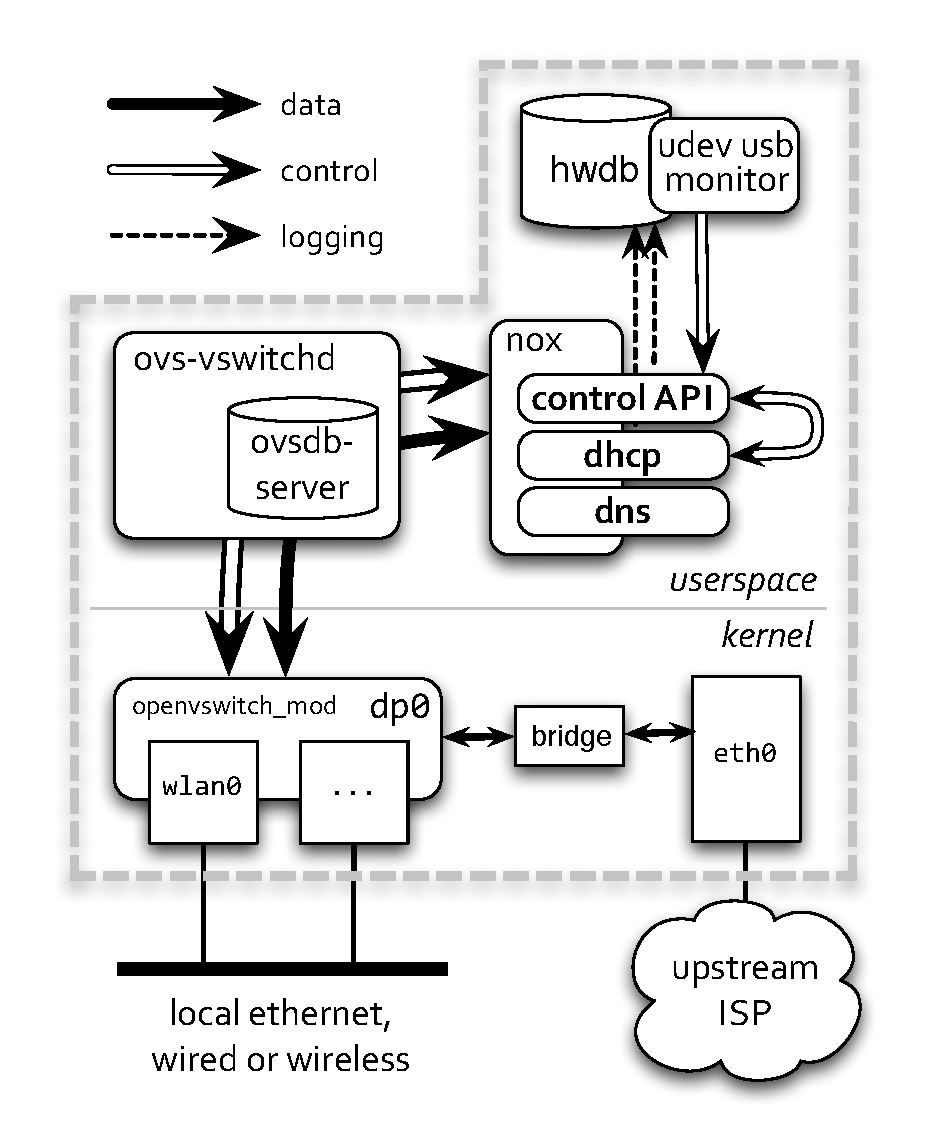
\includegraphics[trim=0.5cm 1cm 0.5cm 2.5cm, width=0.5\columnwidth]{architecture}
  \caption[Home router architecture]{\label{f:architecture}Home router architecture.  \ovs
    and NOX manage the wireless interface.  Three NOX modules
    provide a web services control API, a DHCP server with custom address
    allocation and lease management, and a DNS interceptor, all logging to the
    Homework Database (\emph{hwdb}) (\S\ref{s:protocols}). 
}\end{figure}

Our home router is based on Linux 2.6 running on a micro-PC
platform.\footnote{An Atom 1.6GHz eeePC 1000H netbook with 2GB of RAM running
  Ubuntu 10.04.} Wireless access point functionality is provided by the
\emph{hostapd} package.  The software infrastructure on which we implement our
home router, as shown in Figure~\ref{f:architecture}, consists of the \ovs \of
implementation, a NOX controller exporting a web service interface to control
custom modules that monitor and manage DHCP and DNS traffic, plus the Homework
Database~\mycite{sventek11:_infor_plane_archit_suppor_home_networ_manag} providing
an integrated network monitoring facility.  This gives us a setup very similar
to a standard operator-provided home router where a single box acts as wireless
access point, multiplexes a wired connection for upstream connectivity to the
ISP, and may provide a small number of other wired interfaces. 
                                                                    
We next describe the main software components upon which our router relies.
Using this infrastructure, a number of novel user interfaces was developed, one of
which is described briefly below; details of the others are available
elsewhere~\mycite{mortier11:_suppor_novel_home_networ_manag}.  Note that a key
aspect of our approach is to avoid requiring installation of additional
software on client devices: doing so is infeasible in a home context where so
many different types of device remain in use over extended periods of time.

\subsection{\of, \ovs \& NOX} \label{s:openflow}

We provide \of support using \ovs~\mycite{openvswitch} and employ the
NOX~\mycite{gude08} control platform, an event-driven programmable controller with
C++ and Python module support, to develop our control logic.  Our control logic,
discussed in Section~\ref{s:protocols}, is implemented in five distinct modules.
The C++ module \textit{hwdb} synchronizes router state with the hwdb home
database, presented in Section~\ref{s:hwdb}, the C++ module
\textit{homework\_dhcp} implements our custom DHCP server, the C++ module
\textit{homework\_routing} implements the forwarding logic of the design, the
C++ module \textit{homework\_dns} implements our DNS filtering functionality and
the Python module \textit{homework\_rpc} exposes the control API through a Web
service. 

\begin{table}
  \begin{tabular} {p{0.35\columnwidth}p{0.55\columnwidth}} 
    \textbf{Method} & \textbf{Function} \\ 
    \url{permit/<eaddr>} & Permit access by specified client\\ 
    \url{deny/<eaddr>} & Deny access by specified client\\
    \url{status/[eaddr]} & Retrieve currently permitted clients, or status of specified client \\ 
    \url{dhcp-status/} & Retrieve current MAC--IP mappings\\
    \url{whitelist/<eaddr>} & Accept associations from client\\
    \url{blacklist/<eaddr>} & Deny association to client\\
    \url{blacklist-status/} & Retrieve currently blacklisted clients\\
    \url{permit-dns/<e>/<d>} & Permit access to domain \texttt{d} by client \texttt{e}\\ 
    \url{deny-dns/<e>/<d>} & Deny access to domain \texttt{d} by client \texttt{e}\\ 
  \end{tabular} 
  \caption{\label{t:api}Web service API;
    prefix all methods \texttt{https://\ldots/ws.v1/}.  $<$\,$X$\,$>$ and $[X]$
    denote required and optional parameters.}
\end{table}

Our router provides flow-level control and management of traffic via a single
\of datapath managing the wireless interface of the platform.\footnote{Without
  loss of generality, our home router has only a single wired interface so the
  only home-facing interface is its wireless interface; other home-facing
  interfaces would also become part of the \of datapath.} Control of the router
is provided via a simple web service (Table~\ref{t:api}).  Traffic destined for
the upstream connection is forwarded by the datapath for local processing via
the kernel bridge, with Linux's \emph{iptables} IP Masquerading rules providing
standard NAT functionality.\footnote{While NAT functionality could be
  implemented within NOX, it seemed neither interesting nor necessary to do so.}

%% Without loss of generality, the device we describe in this paper has
%% only a single wired interface so the only home facing interface is its
%% wireless interface, and this is the physical interface managed by the
%% OpenFlow datapath.

\subsection{The Homework Database} \label{s:hwdb}
 
%% \mort{reduce this- it's reported elsewhere: it's a streaming database,
%%  collecting ip layer supporting rpc interaction, and defaults to providing
%%  a Flows table among others; provides the basic measurement
%%  facility accessed by the many uis via rpc}
 
In addition to \ovs and NOX we make use of the Homework Database, \emph{hwdb},
an active, ephemeral stream
database~\mycite{sventek11:_infor_plane_archit_suppor_home_networ_manag}.  The
ephemeral component consists of a fixed-size memory buffer into which arriving
tuples (events) are stored and linked into tables.  The memory buffer is treated
in a circular fashion, storing the most recently received events inserted by
applications measuring some aspect of the system.  The primary ordering of
events is time of occurrence.  

The database is queried via a variant of CQL~\mycite{arasu05:_cql} able to express
both temporal and relational operations on data, allowing applications such as
our user interfaces to periodically query the ephemeral component for either raw
events or information derived from them.  Applications need not be collocated on
the router as \emph{hwdb} provides a lightweight, UDP-based RPC system that
supports one-outstanding-packet semantics for each connection, fragmentation and
reassembly of large buffers, optimization of ACKs for rapid request/response
exchanges, and maintains liveness for long-running exchanges.  Monitoring
applications request can execute temporal query on specific types of events.
\emph{hwdb} also provides notification functionality; applications may register
interest in \emph{future} behaviour patterns and receive notification when such
patterns occur in the database.  The work described in this paper makes use of
three tables: \emph{Flows}, accounting traffic to each 5-tuple flow;
\emph{Links}, monitoring link-layer performance; and \emph{Leases}, recording
mappings assigned via DHCP.

\subsection{The Guest Board} \label{s:guest-board}

\begin{figure} 
  \centering 
  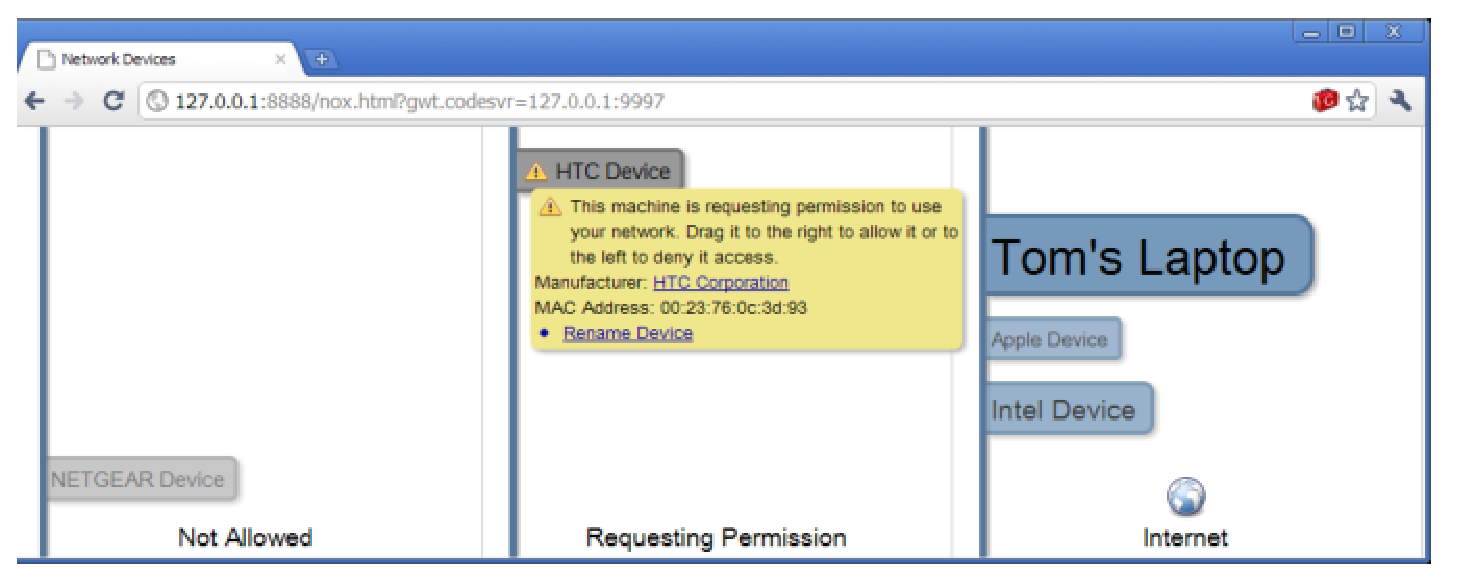
\includegraphics[width=0.9\columnwidth]{homework_guest_board}
  \caption[The \emph{Guest Board} control panel]{\label{f:guest-board}The \emph{Guest Board} control panel, showing an
    HTC device requesting connectivity.}
\end{figure}

This interface exploits people's everyday understanding of control panels in
their homes, e.g.,~heating or alarm panels, to provide users with a central
point of awareness and control for the network. This physical arrangement
provides a focal point for inhabitants to view current network status and to
manage the network.  The interface provides a real time display of the current
status of the network (Figure~\ref{f:guest-board}), showing devices in different
zones based on the state of their connectivity.  The display dynamically maps
key network characteristics of devices to features of their corresponding
labels.  Mappings in the current display are: 

\begin{itemize}
\item Wireless signal strength is mapped to device label transparency, so
      devices supplying weak signals fade into the background.
\item Device bandwidth use is proportional to its label size, e.g.,~Tom's Laptop
      in Figure~\ref{f:guest-board} is currently the dominant bandwidth user. 
\item Wireless Ethernet retransmissions show as red highlights on the device's
  label, indicating devices currently experiencing wireless reliability problems. 
\end{itemize}

Devices in range appear on the screen in real-time, initially in the leftmost
panel indicating they are within range of the home router but not connected.
The central panel in the control displays machines actively seeking to associate
to the access point. This zone exploits the underlying strategy of placing
people in the protocol, discussed in Section~\ref{s:protocols}.  When devices
unknown to the network issue DHCP requests, the router's DHCP server informs the
guest board and a corresponding label appears in this portion of the display.
If a user wishes to give permission for the machine to join the network they
drag the label to the right panel; to deny access, they drag the label to the
left panel. The guest board provides both a central control point and, by
drawing directly upon network information collected within our router, a
network-centric view of the infrastructure. 

\section{Putting People in the Protocol} \label{s:protocols}

We use our home router to enable \emph{ad hoc} control of network policy by
non-expert users via interfaces such as the Guest Board
(Figure~\ref{f:guest-board}).  This sort of control mechanism is a natural fit
to the local negotiation over network access and use that takes place in most
home contexts.  While we believe that this approach may be applicable to other
protocols, e.g.,~NFS/SMB, LPD, in this section we demonstrate this approach via
our implementation of a custom DHCP server and selective filters for wireless
association and DNS that enable management of device connectivity on a
per-device basis. 

Specifically, we describe and evaluate how our router manages IP address
allocation via DHCP, two protocol-specific (EAPOL and DNS) interventions it
makes to provide finer-grained control over network use, and its forwarding
path.  We consider three primary axes: \emph{heterogeneity} (does it still
support a sufficiently rich mix of devices); \emph{performance} (what is the
impact on forwarding latency and throughput of our design and implementation
decisions); and \emph{scalability} (how many devices and flows can our router
handle).  In general we find that our home router has ample capacity to support
observed traffic mixes, and shows every indication of being able to scale beyond
the home context to other situations, e.g., small offices, hotels. 

\subsection{Address Management} \label{s:addresses}

DHCP~\mycite{rfc:2131} is a protocol that enables automatic host network
configuration. It is based on a four way broadcast handshake that allows hosts
to discover and negotiate with a server their connectivity parameters.  As part
of our design we extend the functionality of the protocol to achieve two goals.
First, we enable the homeowner to control which devices are permitted to connect
to the home network by interjecting in the protocol exchange on a case-by-case
basis.  We achieve this by manipulating the lease expiry time, allocating only a
short lease (30 seconds) until the homeowner has permitted the device to connect via a
suitable user interface.  The short leases ensure that clients will keep
retrying until a decision is made; once a device is permitted to connect, we
allocate a standard duration lease (1 hour).

Second, we ensure that all network traffic is visible to the home router and
thus can be managed through the various user interfaces built against it.  We do
so by allocating each device to its own /30 IP subnet, forcing inter-device
traffic to be IP routed via our home router.  This requirement arises because
wireless Ethernet is a broadcast medium so clients will ARP for destinations on
the same IP subnet enabling direct communication at the link-layer.  In such
situations, the router becomes a link-layer device that simply schedules the
medium and manages link-layer security -- some wireless interfaces do not even
make switched Ethernet frames available to the operating system. The result
is that traffic between devices in the
home, such as music distribution and file stores, becomes invisible to the
home router.  By allocating addresses from distinct subnets, all traffic
between clients must be transmitted to the gateway address, ensuring all
traffic remains visible to our home router. 
Our custom DHCP server allocates /30 subnet to each host from 10.2.*.*/16 with
standard address allocation within the /30 (i.e.,~considering the host part of
the subnet, 00 maps to the network, 11 maps to subnet broadcast, 01 maps to the
gateway and 10 maps to the client's interface itself). Thus, each local device
needs to route traffic to any other local device thought the router, making
traffic visible in the IP layer.
%% We deal with the case of
%% misbehaving/malicious clients attempting to subvert our address
%% allocations in~\S\ref{s:association}. 
% \mort{point to lack of perf implications?  or just pull to here?}
%
% The DHCPOFFER generated by our home router in response to a previously unknown
% client allocates a /30 subnet from 10.2.*.*/16 with standard address
% allocation within the /30 (i.e.,~considering the two least significant bits of
% the subnet, 00 maps to the network, 11 maps to subnet directed broadcast, 01
% maps to the gateway and 10 maps to the client's interface itself).  This
% allocation pattern ensures that all traffic for locally connected devices is
% sent via the router, since all devices are on distinct, non-overlapping IP
% subnets.  This would not be the case if addresses were allocated to clients
% from the same subnet, e.g.,~clients were all simply allocated addresses
% directly from 10.*.*.*/8.

We measured the performance of our DHCP implementation and found that, as
expected, per-request service latency scales linearly with the number of
simultaneous requests.  Testing in a fairly extreme scenario, simultaneous
arrival of 10 people each with 10 devices,  gives a median per-host service time
of 0.7 second.

\subsection{Per-Protocol Intervention} \label{s:association}

Our current platform intervenes in two specific protocols providing greater
control over access to the wireless network itself, and to Internet services
more generally. 

\begin{figure} \centering 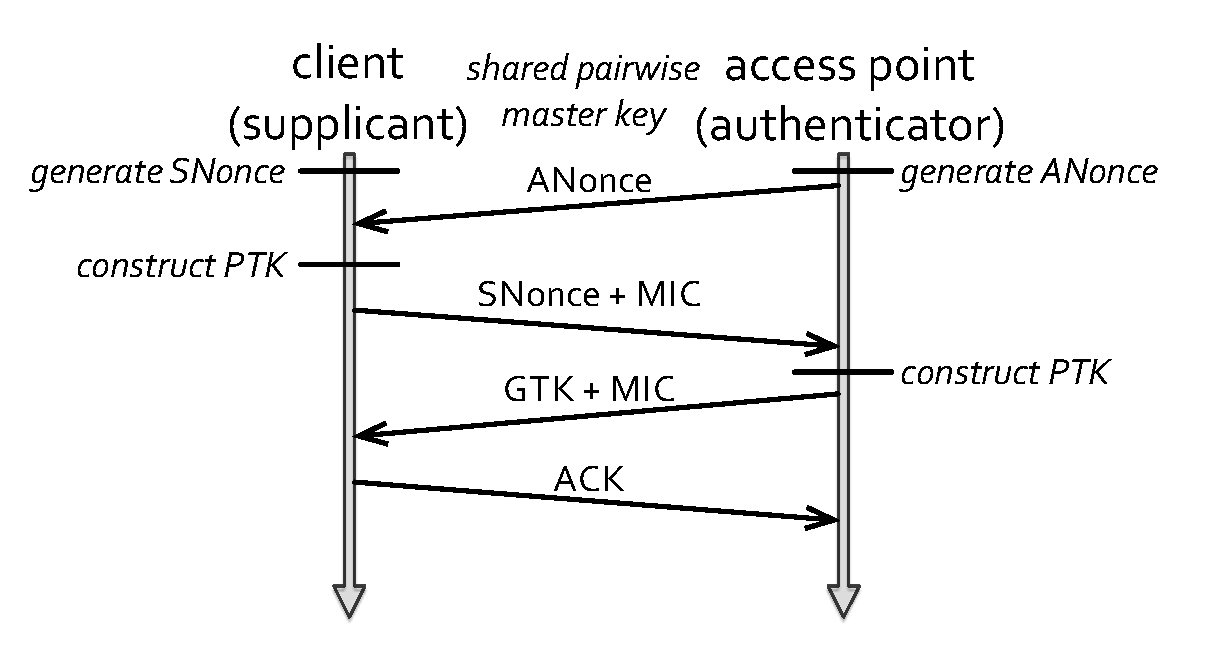
\includegraphics[width=0.8\columnwidth]{eapol}
  \caption[802.11i handshake]{\label{f:association}802.11i handshake, part of the association
    process.  Note that MIC (Message Integrity Code) is an alternate term for
    MAC, used in such contexts to avoid confusion with Media Access Control.}
  \end{figure}
 
Our home router supports wireless Ethernet security via 802.11i with EAP-WPA2,
depicted in Figure~\ref{f:association}, using \emph{hostapd}.  In EAP-WPA2
security mechanism, the
client (\emph{supplicant}) and our router (\emph{authenticator}) negotiate two
keys derived from the shared master key via a four-way handshake, through the
EAPOL protocol.  The \emph{Pairwise Transient Key} (PTK) is used to secure and
authenticate communication between the client and the router; the \emph{Group
  Transient Key} (GTK) is used by the router to broadcast/multicast traffic to
all associated clients, and by the clients to decrypt that traffic.  All
non-broadcast communication between clients must therefore pass via the router
at the link-layer (for decryption with the source's PTK and re-encryption with
the destination's PTK), although the IP routing layers are oblivious to this if
the two clients are on the same IP subnet.\footnote{The 802.11i specification
  defines a general procedure whereby two clients negotiate a key for mutual
  communication (\emph{Station-to-station Transient Key}, STK).  However, the
  only use of this procedure in the specification is in \emph{Direct Link Setup}
  (DLS) used in supporting 802.11e, quality-of-service.  This can easily be
  blocked by the access point, and in fact is not implemented in the
  \emph{hostapd} code we use, so we do not consider it further.
  }

Periodically, a timeout event at the access point initiates rekeying of the PTK,
visible to clients only as a momentary drop in performance rather than the
interface itself going down.  We use this to apply blacklisting of clients
deemed malicious, such as a client that attempts to communicate directly (at the
link-layer) with another client, i.e.,~attempting to avoid their traffic being visible
to our home router.  We wait until the rekeying process begins and then decline
to install the appropriate rule to allow rekeying to complete for the client in
question.  This denies the client access even to link-layer connectivity, as
they will simply revert to performing the four-way handshake required to obtain
the PTK\@.  This gives rise to a clear trade-off between security and performance:
the shorter the rekeying interval, the quicker we can evict a malicious client
but the greater the performance impact on compliant clients.  

\begin{figure} 
  \centering 
  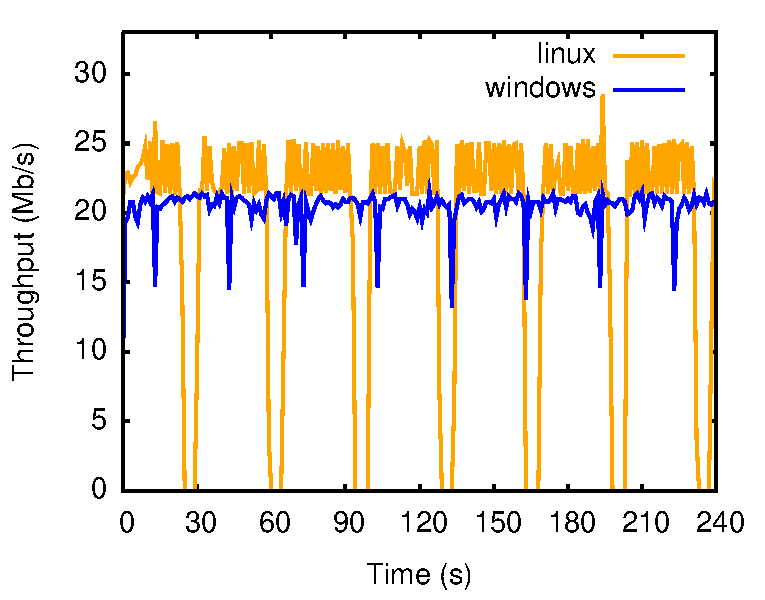
\includegraphics[width=0.5\columnwidth]{Chapter2/Chapter2Figs/rekeying}
  \caption[Affect on TCP throughput from 802.11i rekeying]
  {\label{f:rekeying}Affect on TCP throughput from 802.11i rekeying every 30 seconds
      for Linux 2.6.35 using a Broadcom card with the \emph{athk9} module; and
      Windows 7 using a proprietary Intel driver and card.} 
\end{figure}

\begin{figure*} \centering
 \subfigure[homework switching latency up to 10k concurrent flows]{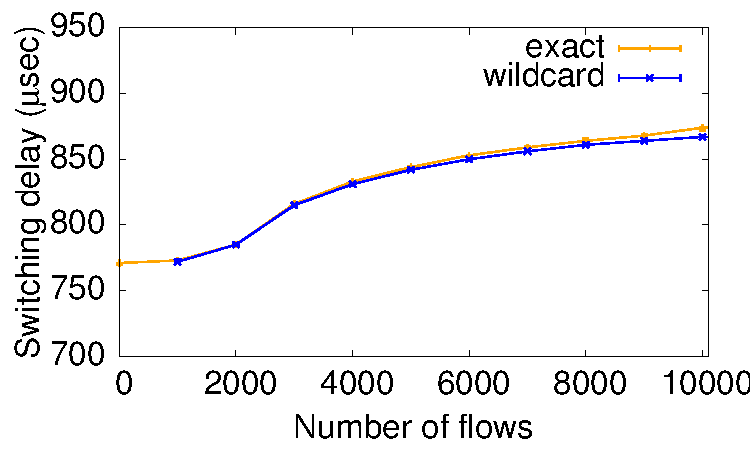
\includegraphics[width=0.45\columnwidth]{Chapter2/Chapter2Figs/latency-test}\label{f:homework:performance-latency-small}}
 \subfigure[homework packet throughput up to 10k concurrent flows]{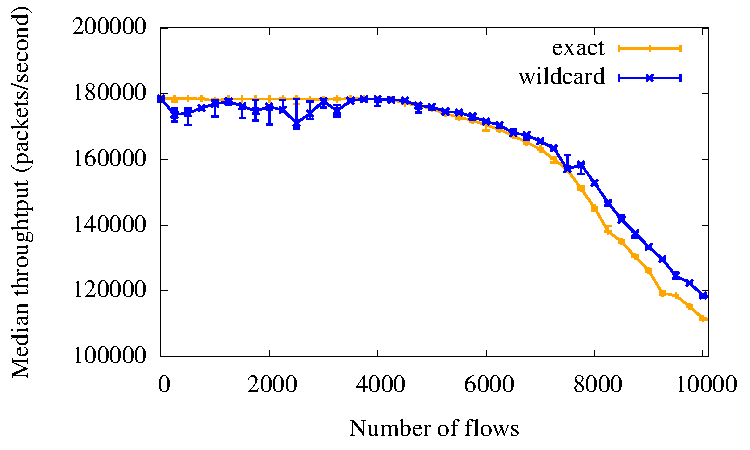
\includegraphics[width=0.45\columnwidth]{Chapter2/Chapter2Figs/throughput-test}\label{f:homework:performance-throughput-small}}
 \subfigure[homework switching latency up to 50k concurrent flows]{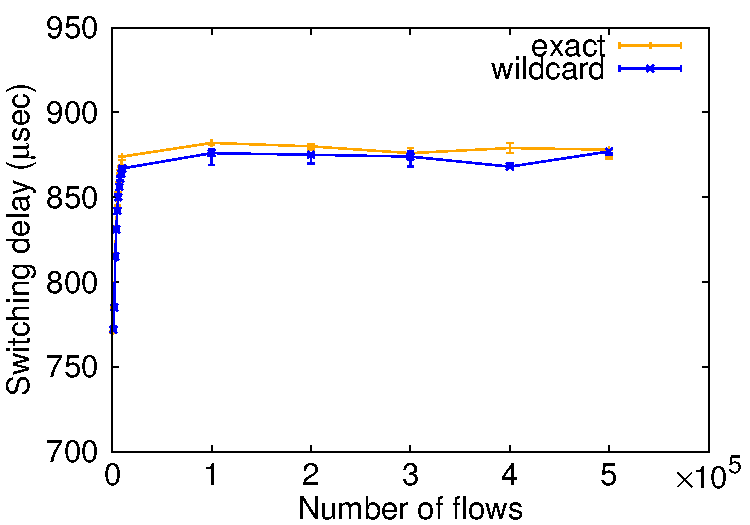
\includegraphics[width=0.45\columnwidth]{Chapter2/Chapter2Figs/latency-large-test}\label{f:homework:performance-latency}}
 \subfigure[homework packet throughput up to 50k concurrent flows]{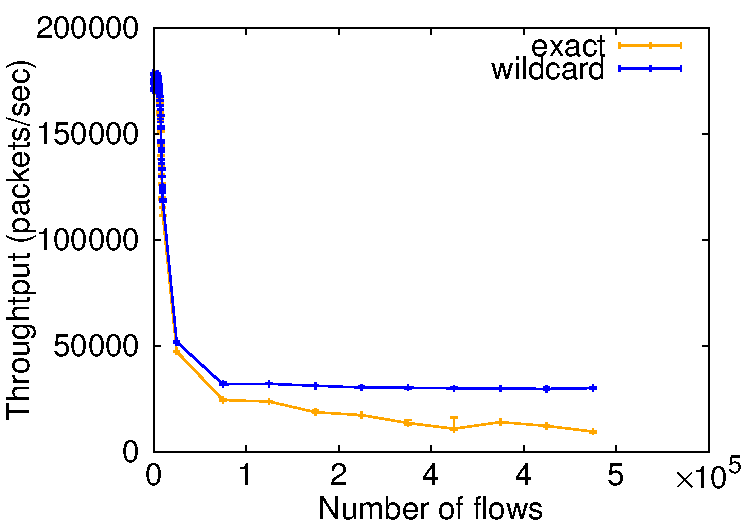
\includegraphics[width=0.45\columnwidth]{Chapter2/Chapter2Figs/throughput-large-test}\label{f:homework:performance-throughput}} 
 \caption[Switching performance of home router]{\label{f:performance}Switching performance of \ovs component
    of our home router showing increasing median per-packet latency
    (Figure~\ref{f:homework:performance-latency},~\ref{f:homework:performance-latency-small}) and
    decreasing median packet throughput
    (Figure~\ref{f:homework:performance-throughput},~\ref{f:homework:performance-throughput-small}) with the number of flows.  The upper set
    of graphs
    (Figure~\ref{f:homework:performance-throughput},\ref{f:homework:performance-latency}) extends the $x$-axis from 10,000 to 500,000.}
\end{figure*}

To quantify the impact of 802.11i rekeying, we observed throughput over several
rekeying intervals.  Figure~\ref{f:rekeying} shows the transient impact to a
steady-state TCP flow of setting the
rekeying interval to 30 seconds: rekeying causes a periodic dip in throughput as the
wireless Ethernet transparently buffers packets during rekeying before
transmitting them as if nothing had happened.  This shows the trade-off between
performance and responsiveness of this approach: to be highly responsive in
detection of misbehaving clients imposes a small performance degradation.  As a
compromise, when a device is blacklisted, all of its traffic and subsequent
rekeying exchanges are blocked.  Thus the misbehaving device is prevented from
sending or directly receiving any traffic before rekeying takes place, The
device will be able to receive only broadcast traffic in the interim due, to the
use of the GTK for such frames, until the AP initiate the negotiation of a new
key.  This allows us to pick a relatively long rekey interval (5 minutes) while
still being able to respond quickly to misbehaving devices.

We also intercept DNS to give fine-grained control over access to Internet
services and websites.  DNS requests are intercepted and dropped if the
requesting device is not permitted to access that domain.  Any traffic the
router encounters that is not already permitted by an explicit \of flow
entry has a reverse lookup performed on its destination address.  If the
resulting name is from a domain that the source device is not permitted to
access, then a rule will be installed to drop related traffic.  Performance is
quite acceptable, as indicated by latency results in Figure~\ref{f:performance}:
the extra latency overhead introduced by our router is negligible compared to
the inherent latency of a lookup to a remote name server.  
% Extending this
% fine-grained control requires more accurate identification of traffic to
% application, particularly for more complex network uses such as BitTorrent and
% Skype, and is a problem we are investigating in ongoing work.

\subsection{Forwarding} \label{s:forwarding}
 
Our router consists of a single \ovs that manages interface
\emph{wlan0}.  \ovs is initialised with a set of flows that push
DHCP/BOOTP and IGMP traffic to the controller for processing.
\ovs by default will also forward to the controller traffic not matched
by any other installed flow, which is handled as follows:

\textbf{Non-IP traffic}.  The controller acts as a proxy ARP server, responding
to ARP requests from clients.  Misbehaving devices are blacklisted via a rule
that drops their EAPOL~\mycite{rfc:3748} traffic thus preventing session keys
negotiation.
% implementing the WPA security association with the access point, so dropping
% it, prevents association.  
Finally, other non-IP non-broadcast traffic has source and destination MAC addresses verified
to ensure both are currently permitted.  If so, the packet is forwarded up the
stack if destined for the router, or to the destination otherwise.  In either
case, a suitable \of rule with a 30 second idle timeout is also installed to
shortcut future matching traffic.

\textbf{Unicast IP traffic}.  First, a unicast packet is dropped if it does not
pass all the following tests: 
\begin{itemize}
    \item its source MAC address is permitted; 
    \item its source IP address is in 10.2.x.y/16; and
    \item its source IP address matches that allocated by DHCP\@.  For valid
      traffic destined to the Internet, a flow is inserted that forwards packets
      upstream via the bridge and IP masquerading.  
\end{itemize} 
Unicast IP traffic that passes but is destined outside the home network has a
rule installed to forward it upstream via the bridge and IP masquerading.  For
traffic that is to remain within the home network a flow is installed to route
traffic as an IP router, i.e.~rewriting source and destination MAC addresses
appropriately.  All these rules are installed with 30 seconds idle timeouts, ensuring
that they are garbage collected if the flow goes idle for over 30 seconds.

\textbf{Broadcast and multicast IP traffic}.  Due to our address allocation
policy, broadcast and multicast IP traffic requires special attention.  Clients
send such traffic with the Ethernet broadcast bit\footnote{I.e.,~the most
  significant bit of the destination address} set, normally causing the hardware
to encrypt with the GTK rather than the PTK so all associated devices can
receive and decrypt those frames directly.  In our case, if the destination IP
address is all-hosts broadcast, i.e., 255.255.255.255, the receiver will process
the packet as normal.  Similarly, if the destination IP address is an IP
multicast address, i.e.,~drawn from 224.*.*.*/4, any host subscribed to that
multicast group will receive and process the packet as normal. Finally, for
local subnet broadcast the router will rebroadcast the packet, rewriting the
destination IP address to 255.255.255.255. This action is required because the
network stack of the hosts filters broadcast packets from different IP subnets.

To assess switching performance, we examine both latency and packet throughput
as we increase the number of flows, $N$, from 1--500,000. In this measurement we
employ a PC, functioning as a data generator and receiver, connected directly
over a 1~Gbps full-duplex Ethernet link to our home route configured to forward all
received packets back to the incoming port. 
% During the experiment, the
% measurement PC uses the pktgen~\mycite{pktgen} kernel module to generate 1 Gbps 
% UDP traffic from a single IP address targeting variable
% number of destination hosts, thus introducing an equivalent number of network
% flows in the network, and measures the processing delay of the router, to
% receive a packet on a port and forward it back the same port. 
Each test runs for two minutes, a sufficient period to observe the network
performance behaviour, generating packets at line rate from a single source to
$N$ destinations each in its own 10.2.*.*/30 subnet, creating equally $N$
unique network flows.  As these are stress tests we use large packets (1500
bytes) for the latency tests and minimal packets (70 bytes)\footnote{The 30
bytes extra overhead is due to \emph{pktgen}~\mycite{olsson05}, the traffic
generation tool used.} for the throughput tests, selecting destinations at
random on a per-packet basis.  Results are presented as the median of 5
independent runs with error bars giving the min and max values. 

Figure~\ref{f:performance} shows median per-packet switching delay and per-flow
packet throughput using either exact-match rules or a single wildcard rule per
host.  Performance is quite acceptable with a maximum switching delay of 560
$\mu$s and minimum throughput of 40000
packets/second~(Figure~\ref{f:homework:performance-latency},\ref{f:homework:performance-latency-small});
initial deployment data suggests a working maximum of 3000 installed flows
which would give around 160000 packets/second throughput (small packets) and
500 $\mu$s switching delay (large
packets)~(Figure~\ref{f:homework:performance-latency-small},\ref{f:homework:performance-throughput-small}).
Using a similar topology we evaluate the performance of multi-homing in Linux
hosts. Figure~\ref{f:stack-throughput} shows that the Linux networking stack is
quite capable of handling the unusual address allocation pattern resulting from
the allocation of each wireless-connected device to a distinct subnet which
requires the router's wireless interface to support an IP address per connected
device. Increasing the number of assigned IP address has no impact on the
processing latency and minimizes marginally the maximum packet processing rate.
This performance behaviour can also be explained by the trie data structure,
used by the Linux kernel to implement longest prefix match, which scale lookup
complexity logarithmically with respect to the number of IP addresses. 

\subsection{Discussion}

Our evaluation shows that \ovs can handle orders of magnitude more rules
than required by any reasonable home deployment.  Nonetheless, to protect
against possible denial-of-service attacks on the flow tables, whether
accidental or malicious, our home router monitors the number of
per-flow rules introduced for each host.  If this exceeds a threshold then
the host has its per-flow rules replaced with a single per-host rule, while the
router simultaneously invokes user interface callback to inform the homeowner of the
device's odd behaviour. 

The final aspect to our evaluation is compatibility: given that our router
exercises protocols in somewhat unorthodox ways, how compatible is it with
standard devices and other protocols?  We consider compatibility along three
separate dimensions: range of existing client devices; deployed protocols that
rely on broadcast/multicast behaviours; and support for IPv6. 

\begin{figure} 
  \centering 
  \subfigure[Packet
  throughput]{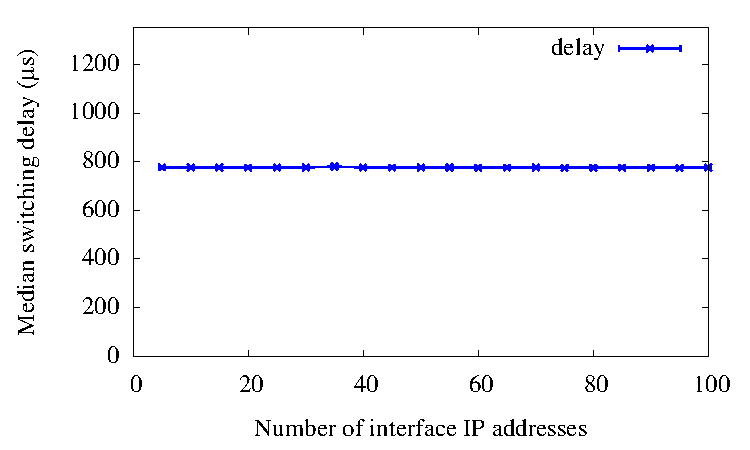
\includegraphics[width=0.49\columnwidth]{Chapter2/Chapter2Figs/stack-throughput-latency}\label{f:homework:stack-throughput}}
  \subfigure[Packet
  latency]{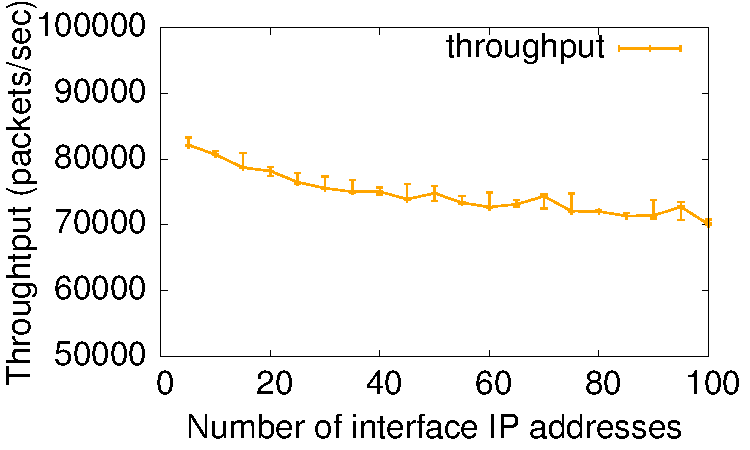
\includegraphics[width=0.49\columnwidth]{Chapter2/Chapter2Figs/stack-throughput-throughput}\label{f:homework:stack-latency}}
  \caption[Switching performance of Linux network]{\label{f:stack-throughput}Switching performance of Linux network
    stack under our address allocation policy. Throughput
    (Figure~\ref{f:homework:stack-throughput}) shows a
    small linear decrease while switching delay
    (Figure~\ref{f:homework:stack-latency}) remains
    approximately constant as the number of addresses allocated to the interface
    increases.} \end{figure}

\paragraph{Devices} Although we exercise DHCP, DNS and EAPOL in unorthodox ways
to control network access, behaviour follows the standards once a device is
permitted access.  To verify that our home router is indeed suitable for use in
the home, we tested against a range of commercial wireless devices running a
selection of operating systems. 

\begin{table*} \centering\footnotesize
  \begin{tabular}{lp{0.33\textwidth}p{0.42\textwidth}} \bf Device & \bf Denied &
    \bf Blacklisted\\

Android 2.x & Reports pages unavailable due to DNS.  & Retries several times
before backing off to the 3g data network.\\

iTouch/iPhone & Reports server not responding after delay based on configured
DNS resolver timeout.  & Requests new wireless password after 1--2 minutes.\\

OSX 10.6 & Reports page not found based on configured DNS resolver timeout.  &
Requests new wireless password after 1--2 minutes.\\

Microsoft Windows XP & Silently fails due to DNS failure.  & Silently
disconnects from network after 4--5 minutes.\\

Microsoft Windows 7 & Warns of partial connectivity.  & Silently disconnects
from network after 4--5 minutes.\\

Logitech Squeezebox & Reports unable to connect; allows server selection once
permitted.  & Flashes connection icon every minute as it attempts and fails to
reconnect.  \\ 

Nintendo Wii & Reports unable to reach server during ``test'' phase of
connection.  & Reports a network problem within 30 seconds.\\

Nokia Symbian OS & Reports ``can't access gateway'' on web access.  & Reports
disconnected on first web access.\\ \end{tabular}
\caption{\label{t:devices}Observed interactions between devices and our home
  router when attempting to access the network.}
\end{table*}

Table~\ref{t:devices} shows the observed behaviour of a number of common
home-networked devices: in short, all devices operated as expected once
permitted access.  DNS interception was not explicitly tested since, as an
inherently unreliable protocol, all networking stacks must handle the case that
a lookup fails anyway.  Most devices behaved acceptably when denied access via
DHCP or EAPOL, although some user interface improvements could be made if the
device were aware of the registration process.  The social context of the home
network means no problem was serious: in practice the user requesting access
would be able to interact with the homeowner, enabling social negotiation to
override any user interface confusion. 

%% We initially investigated using different subnet allocations with
%% short (30 seconds) lease times to more easily distinguish hosts that are
%% trying to connect but are waiting for the homeowner to permit them
%% access.  Unfortunately, due to a variety of issues with common client
%% DHCP implementations, e.g., Android not correctly obeying lease
%% times,\footnote{\url{http://www.net.princeton.edu/android/android-stops-renewing-lease-keeps-using-IP-address-11236.html}} 
%% this broke device interfaces sufficiently that doing so would only
%% increase user confusion.

\paragraph{Broadcast protocols} A widely deployed set of protocols relying on
broadcast and multicast behaviours are those for `zero conf' functionality.  The
most popular are Apple's \emph{Bonjour} protocol; \emph{Avahi}, a Linux variant
of Bonjour; Microsoft's \emph{SSDP} protocol, now adopted by the UPnP forum; and
Microsoft's \emph{NetBIOS}.  

Bonjour and Avahi both rely on periodic transmission of multicast DNS replies
advertising device capabilities via TXT records.  SSDP is similar, but built
around multicast HTTP requests and responses.  We tested Bonjour specifically by
setting up a Linux server using a Bonjour-enabled daemon to share files.  We
observed no problems with any clients discovering and accessing the server, so
we conclude that Bonjour, Avahi and SSDP would all function as expected. 

NetBIOS is somewhat different, using periodic network broadcasts to disseminate
hosts' capabilities.  In doing so we observed a known deficiency of NetBIOS: it
cannot propagate information for a given workgroup between different
subnets.\footnote{\url{http://technet.microsoft.com/en-gb/library/bb726989.aspx}}
However, installing a WINS server on the router mitigates this problem.

In general, it may seem that our address allocation policy introduces link-layer
overhead by forcing all packets to be transmitted twice in sending them via the
router.  However this is not the case: due to use of 802.11i, unicast IP traffic
between two local hosts must \emph{already} be sent via the access point.  As
the source encrypts its frames with its PTK, the access point must decrypt and
re-encrypt these frames with the destination's PTK in order that the destination
can receive them.  Multicast and all-hosts broadcast IP traffic is sent using
the GTK, so can be received directly by all local hosts.  Only directed
broadcast IP traffic incurs overhead which though is a small proportion of the
total traffic; data from a limited initial deployment (about one month in two
homes) suggests that broadcast and multicast traffic combined accounts for less
that 0.1\% (packets and bytes) in both homes.

\paragraph{IPv6 support} 

IPv6 support is once more receiving attention due to exhaustion of the
IPv4 address space.  Although our current implementation does not support IPv6
due to limitations in the current Open vSwitch and NOX releases,\footnote{\of
  provides support in its 1.4 release of the protocol; NOX currently has no
  support for IPv6 and \of versions beyond 1.0; and \ovs only supports IPv6 as a vendor extension of the
  \of protocol.} we briefly discuss how IPv6 would be supported on our
platform.  While these limitations prevent a full working implementation in our
platform, we have verified that behaviour of both DHCPv6 and the required ICMPv6
messages was as expected, so we do not believe there are any inherent problems
in the approaches we describe below.

Addition of IPv6 support affects the network layer only, requiring consideration
of routing, translation between network and link layers, and address
allocation.  Deployment of IPv6 has minimal impact on routing, limited to the
need to support 128~bit addresses and removal, in many cases, of the need to
perform NAT~\footnote{Some operators may still prefer to use NAT as part of a
  legacy of address management and operations.}.  Similarly, supporting
translation to lower layer addresses equates to supporting ICMPv6 Neighbour
Solicitation messages which perform equivalent function to ARP.

Address allocation is slightly more complex but still straightforward.  IPv6
provides two address allocation mechanisms: \emph{stateless} and
\emph{stateful}.  The first allows a host to negotiate directly with the router
using ICMPv6 Router Solicitation and Advertisement packets to obtain network
details, IP netmask and MAC address.  Unfortunately this process requires that
the router advertises a 64 bit netmask, of which current plans allocate only one
per household, with the result that all hosts would end up on the same subnet.
The second builds on DHCPv6 where addresses are allocated from a central entity
and may have arbitrary prefix length.  This would enable our router to function
in much the same manner as currently, although it would need to support the
ICMPv6 Router Advertisement message to support router discoverability by hosts. 

In order to test the functionality, we set up a simple hard-coded version of our
design. Specifically, we allocate a public IPv6 /64 prefix to our home router.
The router uses the ISC DHCPv6 server implementation, configured to allocate
addresses from a /120 subnet.  Additionally, on the router we run the RADVD
daemon to reply appropriately to ICMPv6 messages.  Using this network setup, we
tested MacOSX, Windows and Linux IPv6 network stacks and verified correct network
configuration and Internet connectivity. 


\section{Putting people in the Resource Allocation Policy}\label{s:qos}

\begin{figure}
  \centering
  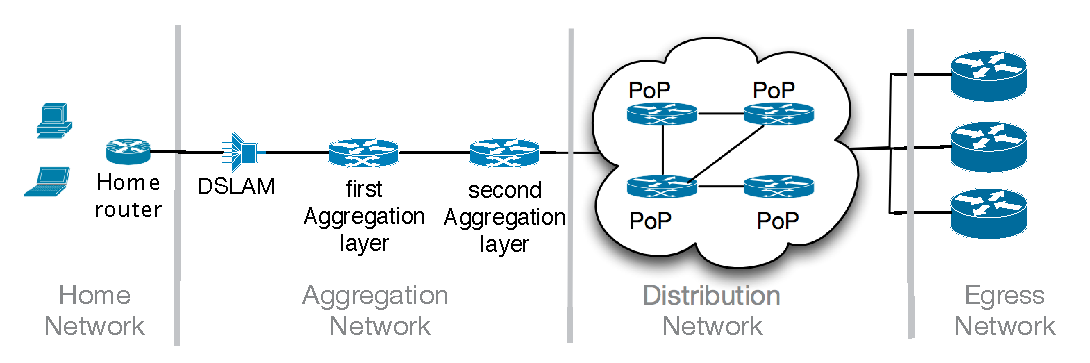
\includegraphics[width=0.95\columnwidth]{isp_plan}
  \caption[ISP network architecture]{\label{fig:isp_plan} ISP network architecture is logically divided in 3
    zones: The {\it Aggregation Network}, the {\it Distribution Network}\/ and
    the {\it Egress Network}.}
\end{figure}

As we have discussed in Section~\ref{sec:intro:net_evolution}, providing strong
performance guarantees in large production networks using commodity technologies
exhibits poor scalability. There are two primary approaches followed by the network
community, to scale resource allocation policies: \emph{network resource
  over-provision}; and \emph{application-aware traffic engineering}.  Resource
over-provision increases available resources thus removing performance
bottlenecks. Application-aware network engineering extends the network
policy to  manage efficiently application traffic, e.g.~VoIP traffic is serviced
by a separate high-priority VLAN\@. Nonetheless, the applicability of these
approaches in broadband networks is limited. On the one hand, resource
over-provision faces a non-scalable deployment cost on the edges of the
network~\footnote{Optical link installation costs vary between \$50-\$200 per
  foot, while fiber installation in municipal areas has an annual cost of \$1.91
  per foot~\mycite{backhaul-cost}. Such upgrades preclude a significant upgrade
  cost for equipment.}, while, on the other hand, application-aware network
engineering raises legal issues for Internet providers~\mycite{hahn06}. In this
section, we propose an architectural extension in the last-mile of the ISP,
enabling homeowners to define per-application resource requirements.  The
architecture improves the ISP resource allocation policy, as well as, the user
experience.  For the rest of this section, we discuss the architecture of
current broadband networks and their  inherent limitations in resource allocation
(Section~\ref{s:qos:motivation}), we present the architecture of our
system (Section~\ref{s:qos:architecture}), and we evaluate its impact on specific
applications classes (Section~\ref{s:qos:eval}).

\subsection{ISP Resource Allocation} \label{s:qos:motivation}

In order to motivate the reader on the benefits of our architecture, we firstly
present the architecture of current broadband networks and identify their
performance bottleneck. Figure~\ref{fig:isp_plan} presents a generic model for
the network architecture for a residential broadband ISP\@. Although, exact
architecture details remain undisclosed, there is a high level design pattern,
organising the ISP network in three domains: the \textit{aggregation network};
the \textit{distribution network}; and the \textit{egress network}. The
aggregation network contains the digital subscriber line access multiplexer
(DSLAM) which translates DSL packets to Ethernet frames, the Broadband Remote
Access Server (BRAS), an authenticating and policy enforcing network service,
and a series of aggregation switches which multiplex traffic between the BRAS and
the distribution network.  Traffic from the aggregation network routes through
the distribution network towards either the egress network or towards a local
aggregation switch. The distribution network consists of a small number of
large routers interconnected using high capacity links.  ISPs typically employ
network tunnelling technologies, like MPLS, in the distribution network to
minimize forwarding state.  The egress network of an ISP consists of large
routers, hosted in Internet Exchange Points (IXP), which connect the ISP with
peering ASes.

A number of research papers have identified a significant bottleneck in the
last-mile of the network~\mycite{Dischinger:2007bg,Akella2003}: the link between
the DSLAM and the aggregation network. This bottleneck can be explained by the
high oversubscription ratio of such links, which commonly varies between 10:1
and 50:1~\mycite{canada-subscription}, depending on population density of an area
and market dynamics~\mycite{sky-oversubscription}.  

Our system aims to bridge a fundamental communication gap between the ISP and
homeowners. Users perceive network traffic as an ensemble of flows belonging to
a specific application and priority class within the home social context,
e.g.~Skype VoIP traffic has a higher priority than web browsing traffic and
parents' teleworking traffic is more important than kids' entertainment
traffic. ISPs view household traffic as a packet aggregate with a specific IP
address, on which resource allocation mechanisms apply monthly or daily traffic
caps~\mycite{virgin-caps,bt-caps}.  Network caps rate-limit heavy-hitting
households and provide long-term fairness between users. Nonetheless, this
approach degrades severely the short-term performance for latency-bound
applications, such as remote desktop and VoIP\@. Effectively, there is an
incentive for ISPs and homeowners to collaborate and control more efficiently
the traffic resources within the user cap.  Homeowners can annotate high
priority flows within their traffic aggregate and thus improve their
experience. ISPs can increase the user-friendliness of their network policy and
offload some of the resource allocation complexity to end-users. 

Our design virtualises network control and resources in the last-mile and
delegates control to a homeowner-managed \of controller.  The household
controller uses the \of protocol to assign traffic flows to appropriate
priority queues.  While the proposed solution cannot always guarantee
end-to-end resource allocation, it provides a sufficient mechanism to handle in
a user-friendly manner edge-network congestion, and scale the configuration
complexity. 

\subsection{Architecture Design} \label{s:qos:architecture}

Congestion in the last-mile requires resource control both in the home network
and within the ISP network. Home traffic is asymmetric and  the network
bottleneck lies beyond the control of the homeowner, thus requiring control on
both traffic directions.  Our architecture consists of three subsystems: a
data-collection daemon on the end-systems of the home network, a \flv
instance in the ISP network translating user flow prioritisation into
forwarding policy, and a policy enforcing daemon on the home network router. 

\paragraph*{Data collection on End-systems}

In order to map network flows to applications, we developed a light cross-platform
daemon recording the content of the end-host connection table.  The daemon
collects mappings between flow tuples and applications names.  Information is
collected from the connection table of the OS and stored in the hwdb database.
The daemon accesses the connection table entries using the
\textit{netfilter-conntrack} library~\mycite{netfilter} in Linux systems, the
\textit{Windows Filtering Platform}~\mycite{win-wfp} in Windows systems and the
\textit{sysctl} for Darwin/MacOSX system.  In order to match each network tuple
with an application, we use the \texttt{lsof} command in Unix-like systems and
the \texttt{netstat -p} command in Windows.


\paragraph*{ISP policy translation}

\begin{figure}
  \centering
  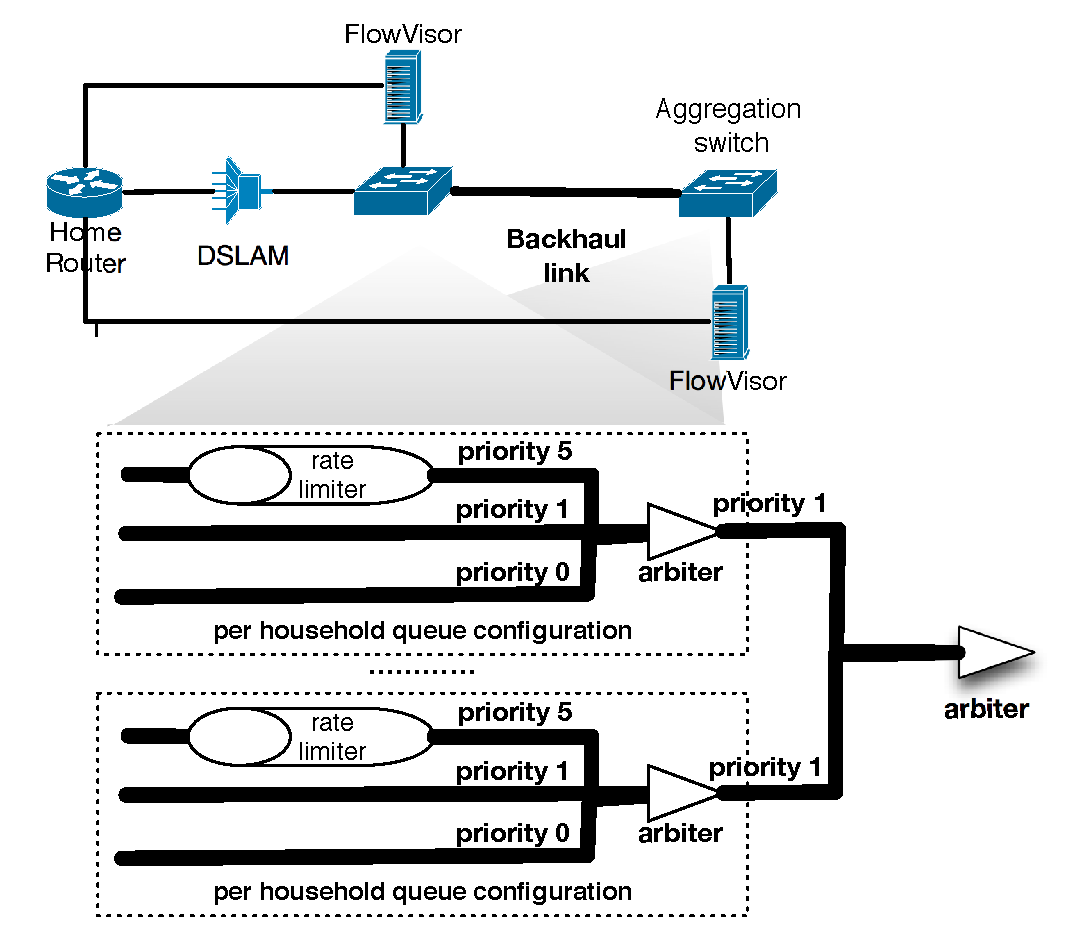
\includegraphics[width=0.7\columnwidth]{queue_design}
  \caption[User-driven QoS architecture]{User-driven network resource allocation architecture. 
    \label{fig:queue_design} A virtual control slice of the downlink between the backhaul
    network and the DSLAM is exposed to each homeowner.  The switch
    uses three queues per-household: A {\it low latency,
      high priority} \/queue, a {\it medium priority} \/queue and a {\it default}
    \/queue.}
\end{figure}

Figure~\ref{fig:queue_design} presents the network architecture of our system.
The resource mechanism exercises control on the home router and on the first layer
of aggregation switches.  The ISP exposes an \of control abstraction which
virtualises switch resources on the aggregation switches using
\flv~\mycite{flowvisor-osdi}, while each home router runs an \of
controller, controlling the home Internet traffic.  The \flv is configured
to provide a clean separation between household control domains in order to
mitigate control or eavesdropping attacks between households. \texttt{pkt\_in}
messages are propagated only to the respective home controller based on IP
addresses, and the home controller can only view and insert flows containing
public IP of the home network\@.   In the household, the resource control mechanism
augments the control logic, presented in the previous section. In order to
minimize forwarding state in the ISP network, the control abstraction on the
aggregation switches is used to control only the incoming Internet traffic,
while the outgoing traffic can be effectively controlled on the local router. 

At the aggregation switch and the home router, we setup three traffic shaping
queues for each household. A \textit{low latency, high priority}~(LLHP) queue, a
\textit{medium priority}~(MP) queue and a default queue.  The LLHP queue has the
highest priority between the household queues and rate limits traffic to the
minimum guaranteed bandwidth per-household~(e.g.~for 1 Gbps uplink with a sharing
ratio of 1:100, the LLHP queue will limit traffic to 10 Mbps), providing strong
low-bandwidth and low-latency guarantees. The MP queue doesn't enforce any rate
limit, but it has a priority which is between the LLHP and the default queue.
MP queue can be used by latency-tolerant high-priority applications.  Finally,
the default queue is used to handle all other traffic types.  The household
queue hierarchies are multiplexed towards the output port using a Round-Robin
scheduler with equal priority for each household. Such large scale queue
hierarchies are currently supported by service provider network equipment
(e.g.~Cisco ASR 9000 routers provide 500000 queues per line
card~\mycite{cisco-asr-qos}) and ISPs use this functionality to implement their
capping policy. By default, all network flows are forwarded to the default queue
and the home \of controller at run-time assigns flows dynamically to higher
priority queues.  The enhanced control of our network architecture
provides some interesting building blocks to enable novel economical models for
residential broadband customers. For example, users can enhance network
performance by purchasing additional flow table entries or by increasing their
minimum guaranteed bandwidth on the edge.

Because our system design provides extensive network control to end-users, we
fortify the design with a set of mechanisms to reduce the possibility
of network functionality compromise.  Firstly, fair allocation of flow table
entries to each household, ensures fair utilisation of the forwarding resources
in the aggregate switch. Secondly, the \flv instance rate limits \of
control channel interactions per household to mitigate DoS attacks. Finally, the
\flv instance discards flows that may create loops in the network,
e.g.~flow rules that forwards packet to the incoming port. 

\paragraph*{Home \of controller}

\begin{figure}
  \centering
  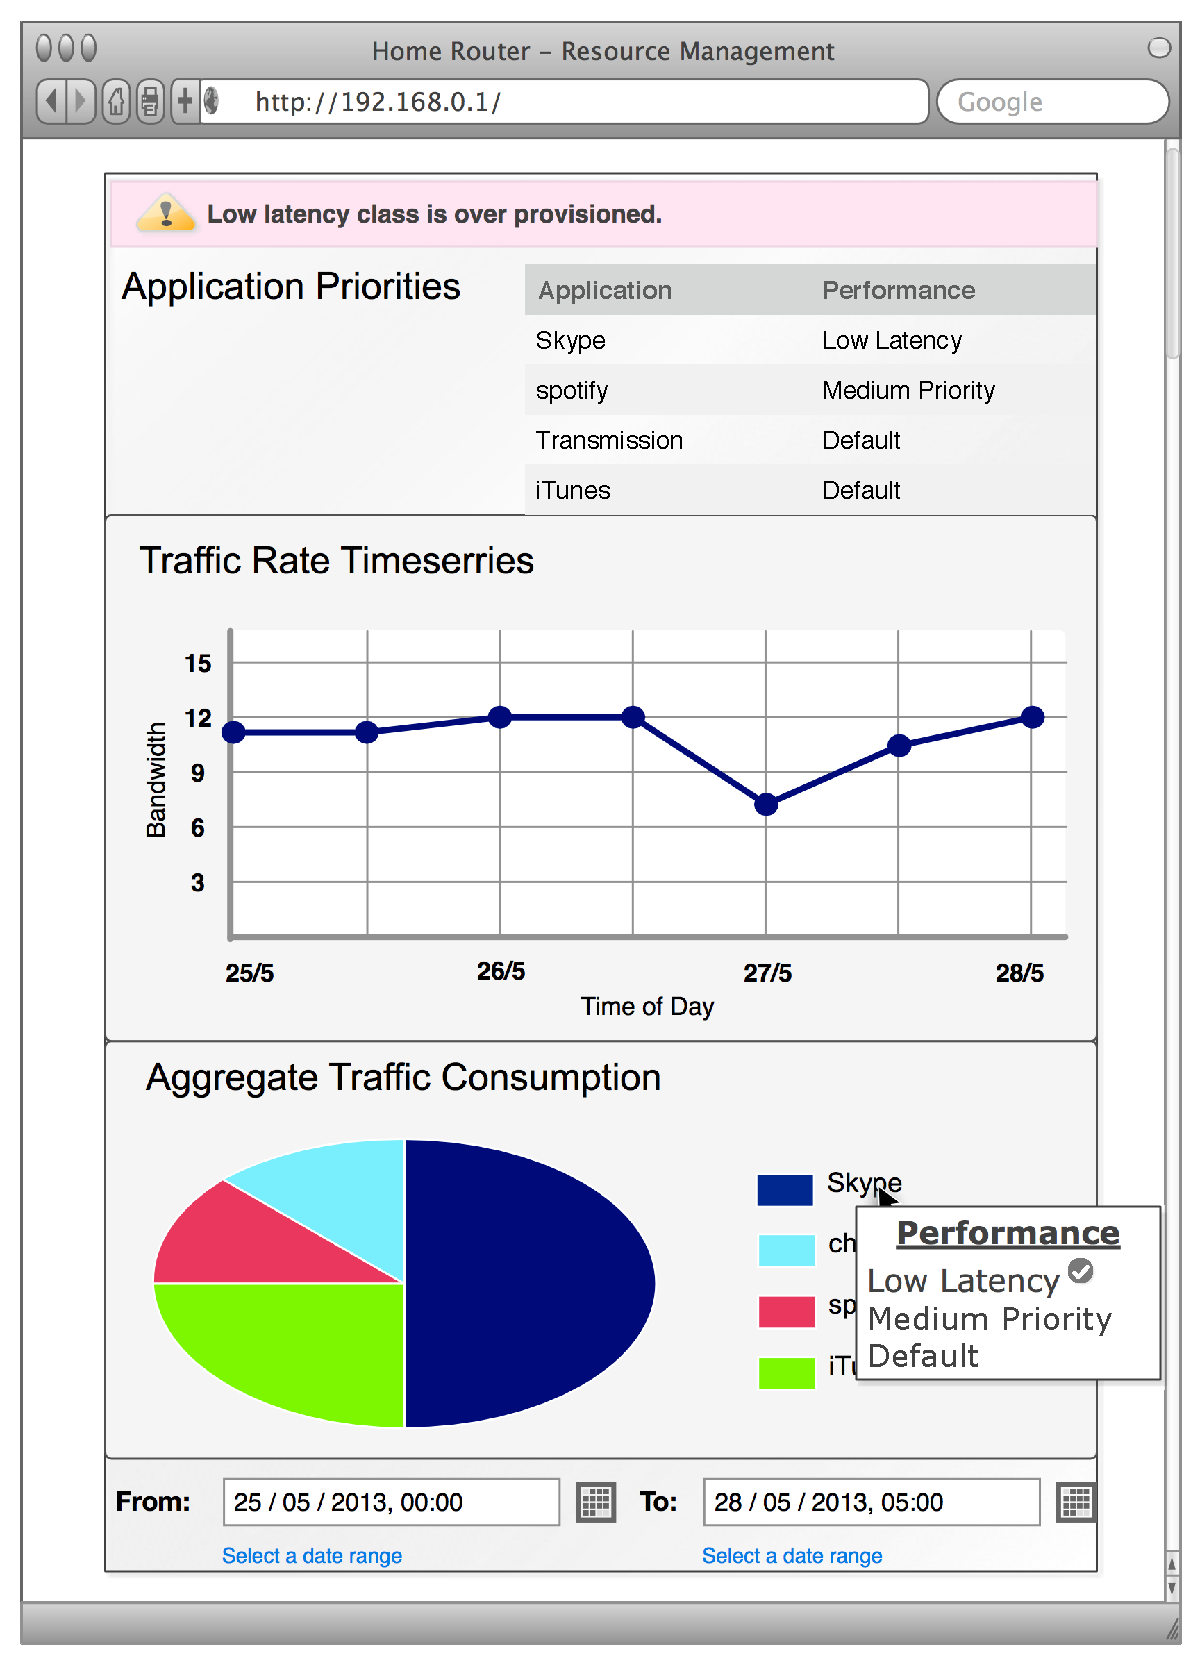
\includegraphics[width=0.8\columnwidth]{homework_intf_qos}
  \caption[QoS user interface]{\label{fig:homework_intf_qos} QoS user interface.
    The user is able to view the network utilisation per application, as well as
    express application prioritisation.}
\end{figure}

In our design, the home router is the rendez-vous point between the policies of
the two entities, responsible to store traffic statistics, record the user
application priority, and at run-time map application flows to the appropriate
queue.  We use three tables in HWDB to store relevant information:
\texttt{application tuple}; \texttt{application timeseries}; and
\texttt{application priority}; tables.  The~\texttt{application tuple} table
stores mappings between applications and flow tuples populated with data from
the data-collection daemon.  The~\texttt{application timeserries} table stores
the per-application network utilization, populated with router data
using~\texttt{flow\_stats} messages.  Finally, the~\texttt{application
priority} table stores the user's application prioritisation policy. 

We expose resource control of our system to home members through a web
interface, presented in Figure~\ref{fig:homework_intf_qos}.  The interface
presents the aggregate and timeserries resource consumption for each
application, using the data of the \texttt{application timeseries} table, and
enables control of application prioritisation. Additionally, the interface
notifies the user when the policy over-utilises the LLHP queue.  Specifically,
the packet loss counter from the \of~{\tt queue\_stats} message is used to detect 
high packet loss incidents.  Through this interface, we
address issues raised by~\mycitet{Chetty10}. 

During operation, the proposed design extends the forwarding logic described
earlier. Specifically, each valid network flow destined to a non-local host is
mapped to an application, through the \texttt{application tuple} table,  and to
a priority queue, through the \texttt{application priority} table. The
controller sends a {\tt flow\_mod} message with an {\tt enqueue} action to
assign the flow to the appropriate queue. In addition, if the application
priority is not the default, then the controller will also send a {\tt
flow\_mod} packet to the \flv instance to setup the incoming direction of
the flow. 

\subsection{Evaluation} \label{s:qos:eval}

\begin{figure}
  \centering
  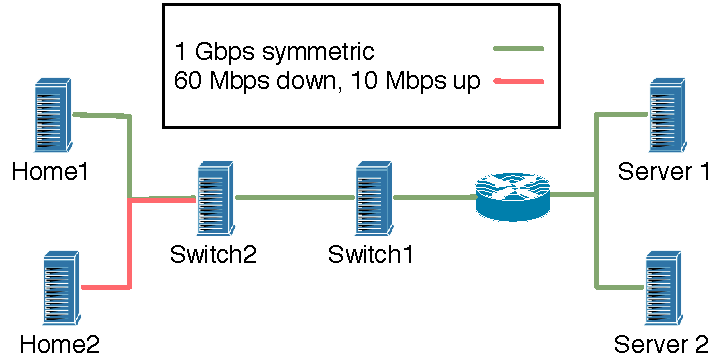
\includegraphics[width=0.6\columnwidth]{queue_eval_setup}
  \caption{\label{fig:queue_eval_setup} QoS mechanism evaluation topology.}
\end{figure}

\begin{table}
    {\small
  \begin{tabular} {|l|c|l|c|}
    \hline
    \multicolumn{2}{|c|}{\textbf{Web traffic}} & \multicolumn{2}{|c|}{\textbf{Gaming traffic}} \\
    \hline
    \textbf{Parameter} & \textbf{Distribution} & \textbf{Parameter} & \textbf{Distribution} \\
    \hline
    objects per page    & Pareto(2.43, 3.00)       &                  &                       \\
    inter-request delay & Pareto(1.50, 0.75)       & inter-packet gap & Lognormal(79.34, 0.25)\\
    inter-object delay  & Weinbull(1.46, 0.38)     & packet size      & Constant(0.05)        \\
    object size         & Lognormal(1.31, 9.35)    &                  &                        \\
    
    \hline
  \end{tabular} 
 } \caption{\label{t:homework:performance-web-model}Model parameters for HTTP~\mycite{Barford1998} and
    gaming~\mycite{Lang2004} traffic generation.}
\end{table}


In this section, we evaluate the impact of our architecture on
performance-sensitive applications.  Figure~\ref{fig:queue_eval_setup} presents
the topology we employ for our evaluation.  \textit{Home1} and \textit{Home2}
emulate household Internet traffic,  \textit{Server1} and \textit{Server2}
emulate Internet services,  \textit{Switch1} emulates the last-mile of the ISP
network and \textit{Switch2} emulates the Internet path between the aggregation
layer of the ISP and the Internet services. In detail, Home1 emulates a single
household running a resource critical application towards Server1, while Home2
emulates an ensemble of nine households generating bursty HTTP requests towards a
web service on Server2, using the web model in
Table~\ref{t:homework:performance-web-model}.  Switch1 provides asymmetric
Internet links with 4 Mbps downlink capacity and  512 Kbps uplink capacity to
each household and  connects them to the ISP distribution network through a 4
Mbps symmetric link, thus providing a downstream subscription ratio $1:10$.
Switch2 propagates traffic between Switch1, Server1 and Server2, adding 10~ms
of one-way latency to each direction. Each node in the  topology runs on a
different host equipped with a quad core Intel CPU (Core 2 Quad Q6600), 4 GB
RAM and a quad-port 1 GbE Intel card. Switch1 and Switch2 use \ovs to implement
fast packet forwarding functionality.

Using the aforementioned topology, we evaluate the impact of our architecture
on two popular applications, VoIP and Gaming. Without loss of generality, the
selected applications provide a representative set in terms of  latency and
throughput requirements.  We emulate VoIP traffic, using a constant rate 250
Kbps TCP
flow~\footnote{\url{https://support.skype.com/en/faq/FA1417/how-much-bandwidth-does-skype-need}},
while for gaming traffic we use a UDP probe based on the model presented in
Table~\ref{t:homework:performance-web-model}. We conduct the measurement for
300 seconds, initializing the network without any traffic prioritisation, and
we enable our architecture after 150 seconds of execution, assigning the HTTP
application on the default queue and the VoIP and Gaming applications on the
LLHP queue. Figures~\ref{f:homework:performance-qos-gaming}
and~\ref{f:homework:performance-qos-voip} present the results of the experiment
for the gaming and VoIP applications respectively. More specifically, we
present the per-packet latency for gaming and the instantaneous
application-perceived throughput for VoIP, along with the instantaneous
aggregate throughput of all HTTP flows. For the gaming application, we observe
that packets face significant latencies (200-500 ms), primarily due to
queueing delays when they coexisting in a congested link with HTTP flows and
the network is not using any short-term resource control. The latency is
effectively minimized when we enable our architecture without significant
performance degradation for HTTP traffic. Similarly, VoIP traffic experiences
significant throughput variations (200-350 Kbps) which are eliminated when the
flow is assigned to the LLHP queue.  The results verify that the proposed
short-term resource control mechanism can significantly improve user
experience and effectively improve network performance for applications
with strict resource requirements, while introducing minimal impact on
the performance of less critical flows.
%co-existing application performance. 

\begin{figure*} \centering
 \subfigure[Gaming]{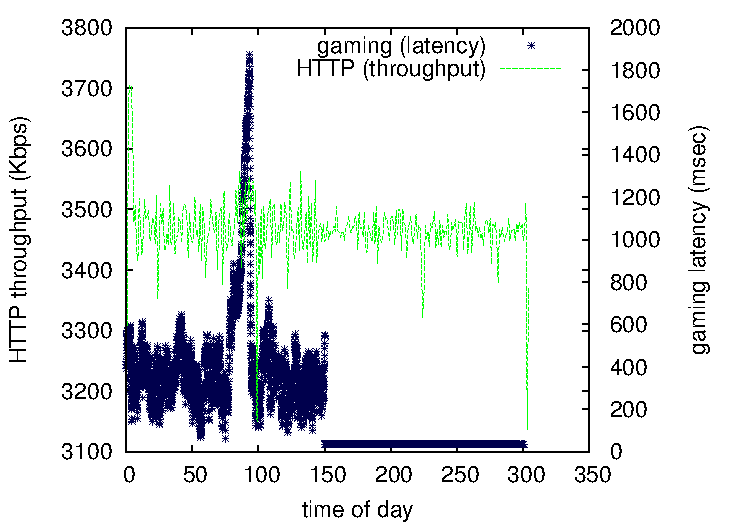
\includegraphics[width=0.49\columnwidth]{Chapter2/Chapter2Figs/homenet-prio-gaming}\label{f:homework:performance-qos-gaming}}
 \subfigure[VoIP]{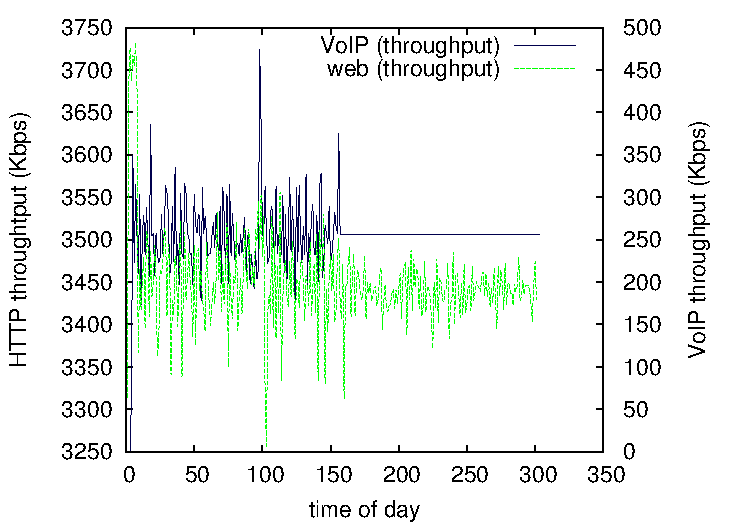
\includegraphics[width=0.49\columnwidth]{Chapter2/Chapter2Figs/homenet-prio-voip}\label{f:homework:performance-qos-voip}}
 \caption[QoS mechanism Latency and throughput evaluation]{\label{f:homework:performance-qos} Latency and throughput performance
  of the QoS architecture. The QoS mechanism is enabled after 150 seconds of
  execution, reducing significantly packet latency and providing accurate
  throughput bounds.}
\end{figure*}

\section{Summary} \label{s:conclusion}

This chapter has drawn upon previous user studies to reflect on the distinct
nature of home networks and the implications for domestic network
infrastructures.  Three particular user needs that arose from home network user
studies were for richer visibility into and greater control over the home
wireless network, as well as the home as part of the everyday management of the
home by inhabitants.  We  considered how to exploit the nature of the home
network in order to shape how it is presented and opened to user control and
ultimately to provide scalable management through a novel control plane
architecture.  

We used the \ovs and NOX platforms to provide flow-based management of the home
network.  As part of this flow-based management, we exploited the social
conventions in the home to manage introduction of devices  to the network, and
their subsequent access to each other and Internet hosted services.  This
required modification of three standard protocols, DHCP, EAPOL and DNS, albeit
in their behaviour but \emph{not} their wire formats, due to the need to retain
compatibility with legacy deployed stacks. In addition, in our exploration we
presented a simple mechanism enabling home user to guide the ISP resource
allocation mechanism in order to fulfil application requirements.  Our
exploration, on one hand, provides strong evidence that appropriate design of
the control plane architecture can transform and scale the management effort,
while on the other hand, it suggests that existing presumptions could usefully
be re-examined to see if they still apply in a network context.  In the next
chapter we explore application of SDN technologies in naming and connectivity
scalability. 

% \section{Technological and Social aspects of home networking} \label{s:elephant}
% 
% The growth in the number of IP-enabled devices over the last decade  has
% expanded the use-cases for in-home wired and wireless networking; from Internet
% connection sharing to local media sharing, gaming, and other applications.  Home
% network functionality, unlike other network environments, contains a strong
% social aspect, which establishes a dynamic relationship between the technology
% and the social organisation of the setting, exhibiting some unique properties.
% In this Section, we summarize finding of relevant studies and elaborate on the
% characteristics of home network environments, both from a social and an
% engineering perspective.  More specifically, in Section~\ref{s:home_measurement}
% we present the distinct technical characteristics of home network technologies,
% while in Section~\ref{s:home_social} we focus on the social characteristics of
% home networking, using findings from relevant ethnographic studies. 
% 
% \subsection{Home Networking as a system} \label{s:home_measurement}
% 
% Home networks are highly heterogeneous edge networks, typically
% Internet-connected via a single broadband link, where non-expert network
% operators provide a wide range of services to a small set of users.
% While we focus on home networks, we note that many environments, e.g.,~small
% offices, coffee shops, hotels, exhibit similar characteristics and thus may
% benefit from similar approaches. Such capabilities are likely to be infeasible
% in more traditional settings, e.g.,~backbone and enterprise networks.  In this
% section we use existing studies to present the technical characteristics of
% modern home network. 
% % More specifically, we present the type of devices
% % connected to a home network, the properties of the local and Internet traffic
% % and the properties of local and Internet connectivity. 
% 
% % Home network measurement studies have focused both on the local network
% % properties as well as the nature of the Internet traffic. Local network analysis
% % provides useful insight on the way devices interact within the house and the
% % possible performance limitations. Such measurement studies focused mainly on
% % developing active or passive measurement tools, that runs on end-hosts in the
% % network and collect data. 
% Home networks commonly provide local device connectivity through wired and
% wireless Ethernet, both supported by modern PCs. Wired network adapters
% predominantly support the 802.3ab (1 Gbps full-duplex) standard and wireless
% network adapters support predominantly 802.11a/g (54 Mbps) standards, while
% 802.11n (600 Mbps) support is slowly increasing.  Wired Ethernet connectivity
% provides high data rates with negligible medium interferences, but fails in
% supporting flexible spatial mobility within the household. In contrast, wireless
% Ethernet connectivity supports extensive device mobility, but network
% performance is susceptible to environmental parameters.  \mycite{homenetProfiler}
% study the availability of wireless connectivity in home networks and report on
% average good signal coverage~($<$ -80dBm), verifying a significant technological
% improvement which overcomes connectivity problem highlighted by earlier
% studies~\mycite{Yarvis05characterizationof}. In addition, the authors observe
% significant wireless network overhearing,  with end-hosts  picking up 10
% wireless networks on average, a third of which used overlapping channels.  The
% accessibility of wireless networks beyond the physical home  limits highlights a
% significant access control problem. The WPA encryption scheme, used
% predominantly to mitigate this problem, ensures network data integrity but lucks
% flexibility; pre-shared key knowledge provides full access to the home network.
% 
% Home networks use predominantly ADSL and cable technologies to provide Internet
% connectivity, while fiber, 3G and satellite technologies are not uncommon. As a
% result, Internet connectivity exhibits high variance in performance, depending
% extensively on the medium and the ISP\@.  \mycite{Dischinger2007} present an early
% broadband performance study, reporting significant performance variance and a
% bottleneck on the last mile of the link.  \mycite{Sundaresan2011} contact a
% similar studies, running though measurements probes on the home router, and
% detect significant effects on network throughput and latency by ISP throttling
% mechanisms, like PowerBoost~\mycite{powerboost}. Finally, \mycite{Kreibich10} verify
% the bufferbloat problem in residential broadband ISPs.  The importance of
% Internet performance for residential broadband networks is reflected on a
% governmental level, where independent state authorities evaluate ISP service
% quality~\mycite{fcc, ofcom}.  
% 
% Home networks exhibit unique applications and traffic characteristics.
% \mycite{Reggani12} contact an in-network passive measurement and study the host
% network behaviour, under different network environments. The study concludes
% that in the home network end-hosts exhibits a distinct network behaviour,
% generating high volumes of filesystem and P2P applications, while a significant
% portion of the traffic remains local.  Residential broadband Internet traffic
% patterns exhibit significant temporal and spatial variability.  \mycite{Cho2006}
% detect in 2005 significant volumes of P2P traffic in Japanese bradband ISPs.
% More recently, \mycite{Maier2009} analyse traffic traces from a German ADSL
% provider and detect a significant shift towards web applications.
% \mycite{Erman2011} detect similar trends in US broadband traces, identifying more
% that 70\% of the network traffic being HTTP and serving primarily online video
% and one-click hosting services. 
% 
% In terms of device demographics, relevant studies identify an increase in the
% number and heterogeneity of connected devices. \mycite{homenetProfiler} present a
% user survey reporting that home networks host on average 7-8 devices. In
% addition, the users report wide variability in connected devices
% (e.g.~smartphones, tablets, game consoles, etc.), highlighting a strong openness
% requirement in any modification in the network functionality.  Nonetheless,
% \mycite{Hatonen10} test off-the-self home routers and unveil high variability in
% the semantics of the NAT and DNS implementations.  Since such routers are widely
% deployed in home networks, applications remain robust towards this variability.
% % to consider this variability as acceptable. 
% % widespread usage of such routing kit, the impact to home networking appears to be
% % minimal and home network environment appears to be resilient to non-standard
% % router implementations. 
% 
% \subsection{Home Network as a social activity} \label{s:home_social}
% 
% Home networks technologies provide an excellent setting to study the
% interactions of social behaviours and technology.  Studies in the field usually
% engage in user interviews in order to understand how users perceive and interact
% with network technologies. 
% 
% An important aspect in analysing the home network from a social aspect, requires
% an in-depth understanding of the user perception of  home network technologies.
% \mycite{shehanpoole08,grinter05} analyse user sketches presenting their network
% technology understanding and highlight two important observations; user opacity
% to the network increases inversely proportional to their user network experience
% -- verifying the effectiveness of the network abstraction, and users identify
% network devices using the social context of the home network.  Further,
% \mycite{tolmie07} perform an empirical analysis of the home member interactions
% with network technologies. Their finding point out that users appear reluctant
% to optimize network configuration, while they experience tolerable performance.
% Such tasks though can become more elegant if they have small duration and
% consist of well-defined steps. Furthermore, interest conflicts, arising due to
% resource sharing, are usually solved through negotiation between household
% members. Furthermore, relevant studies have highlighted the importance of
% accurate information of the utilization and state of the network for network
% management. \mycite{Chetty10} analyse the effect of bandwidth utilization
% visualisation in user experience, reporting improved user understanding of
% network functionality and troubleshooting, but also raised privacy concerns. 
% 
% Home network configuration and management are influenced to a great extend by
% the design of the house and the routines of the house members.  \mycite{Rodden03}
% use the~\mycite{Brand94} model of home architecture temporal evolution, to analyse
% the relationship between ubiquitous technologies and home design and understand
% the interactions between home design and network usage. The study reports that
% network decisions are severely affected by the design of the house, e.g.,
% location of the network router, while at the same time, users confuse the limits
% of the house with the limits of their network, e.g.~users declare wireless
% encryption as irrelevant, since it is contained within the limits of the house.
% % In~\mycite{rodden04,crabtree03} the authors monitor the real time communications
% % and information flows in a multi-member household. The study concludes that
% % communication activities have a location reference defined to the involved
% % member as well as the house planning, while activities can be synthesized as
% % sequences into higher order activities. Additionally, using these
% % observations, they propose a framework which can model such interactions. 
% In addition, \mycite{shehan07} analyse common management and configuration
% problems in home networks and draw parallels with respective design decisions in
% the network systems.  They present a weight of evidence, pointing out that
% problems with current network technologies are not amenable to solution via a
% `thin veneer' of user interface technology layered atop the existing
% architecture.  Rather, they are \emph{structural}, emerging from the mismatch
% between the stable `end-to-end' nature of the Internet and the highly dynamic
% and evolving nature of domestic environments.  
